\documentclass[aspectratio=169]{beamer}
\PassOptionsToPackage{english}{babel}
\usepackage{standardslides}

\def\UrlBigBreaks{\do\/\do-\do:}

\title{Restricted Boltzmann Machines}
\author{Markus Pawellek}

\DeclareMathOperator{\sigm}{\mathrm{sigm}}
\DeclareMathOperator{\expect}{\mathds{E}}
\begin{document}
  \selectlanguage{english}
  % \urlstyle{sf}
  \renewcommand{\separate}{\qquad}

  \begin{frame}
    \vfill
    
\includegraphics[width=\textwidth]{images/netflix-logo.jpg}
    \vfill
  \end{frame}

  \frame{\titlepage}
  \begin{frame}{Outline}
    \footnotesize
    \hfill\parbox[t][7cm][l]{0.9\textwidth}{\tableofcontents}
  \end{frame}

  \section{Problem} % (fold)
  \label{sec:Problem}
    \begin{frame}{Problem: Collaborative Filtering -- Movie Ratings}
      \begin{center}
        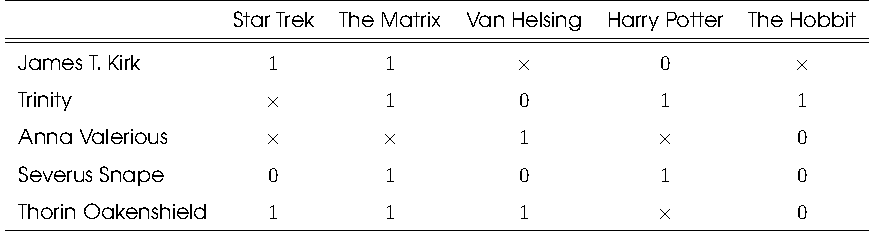
\includegraphics[height=0.35\textheight]{figures/problem-example.pdf}
      \end{center}
      \vfill
      \pause
      Goal:
      \begin{itemize}
        \pause
        \item approximately represent a complex probability distribution
        \pause
        \item learn probability distribution based on given samples
        \pause
        \item make predictions based on learned parameters
      \end{itemize}
    \end{frame}
  % section Problem (end)

  \section{The Model} % (fold)
  \label{sec:The Model}
    \begin{frame}{The Model: Idea}
      \vfill
      \begin{center}
        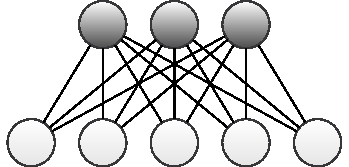
\includegraphics[scale=1.6]{figures/rbm-scheme-empty.pdf}
      \end{center}
      \vfill
    \end{frame}

    \begin{frame}{The Model: Idea}
      \vfill
      \begin{center}
        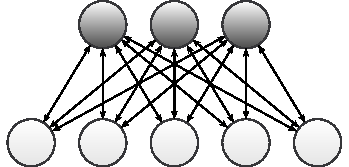
\includegraphics[scale=1.6]{figures/rbm-scheme-arrows.pdf}
      \end{center}
      \vfill
    \end{frame}

    \begin{frame}{The Model: Idea}
      \begin{center}
        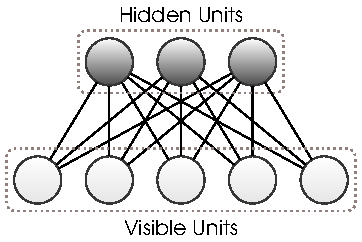
\includegraphics[scale=1.2]{figures/rbm-scheme-layers.pdf}
      \end{center}
      \begin{itemize}
        \pause
        \item units are divided into two subsets
        \pause
        \item only connections between hidden and visible units are allowed
      \end{itemize}
    \end{frame}

    \begin{frame}{The Model: Idea -- Inputs}
      \vfill
      \begin{center}
        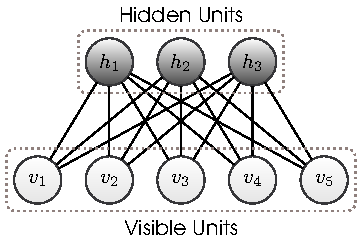
\includegraphics[scale=1.6]{figures/rbm-scheme-inputs.pdf}
      \end{center}
      \vfill
    \end{frame}

    \begin{frame}{The Model: Idea -- Example}
      \vfill
      \begin{center}
        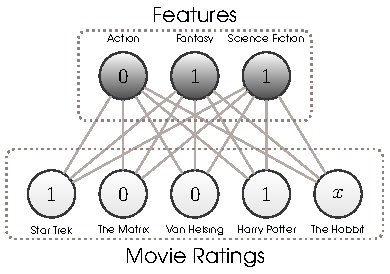
\includegraphics[scale=1.6]{figures/rbm-scheme-example.pdf}
      \end{center}
      \vfill
    \end{frame}

    \begin{frame}{The Model: Parameters}
      \begin{center}
        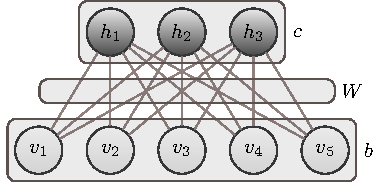
\includegraphics[scale=1.2]{figures/rbm-scheme.pdf}
      \end{center}
      \pause
      \begin{mybox}
        \[
          v \in V \define \set{0,1}{}^n
          \separate
          h \in H \define \set{0,1}{}^m
          \separate
          ϑ \define (W,b,c) \in \setReal^{(n\times m) + n + m}
        \]
      \end{mybox}
    \end{frame}

    \begin{frame}{The Model: Probability Distribution and Energy}
      \begin{mybox}
        \[
          \function{p[ϑ]}{V\times H}{[0,1]}
          \separate
          p[ϑ](v,h) \define \frac{e^{ -E[ϑ](v,h) }}{Z(ϑ)}
        \]
      \end{mybox}
      \pause
      \vfill
      \begin{mybox}
        \[
          \function{E[ϑ]}{V\times H}{\setReal}
          \separate
          E[ϑ](v,h) \define -\transpose{v}Wh - \transpose{v}b - \transpose{h}c
        \]
      \end{mybox}
      \pause
      \vfill
      \begin{mybox}
        \[
          Z(ϑ) \define \sum_{v\in V} \sum_{h\in H} e^{ -E[ϑ](v,h) }
        \]
      \end{mybox}
    \end{frame}

    \begin{frame}{The Model: Probability Distribution for Visible Units}
      \begin{mybox}
        \[
          \function{p[ϑ]}{V}{[0,1]}
          \separate
          p[ϑ](v) \define \sum_{h\in H} p[ϑ](v,h)
        \]
      \end{mybox}
    \end{frame}

    \begin{frame}{The Model: Posterior Probability}
      \begin{center}
        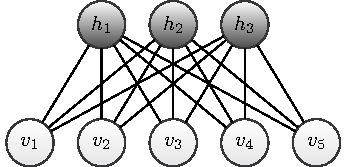
\includegraphics[scale=1.2]{figures/rbm-scheme-inputs-only.pdf}
      \end{center}
      \pause
      \begin{mybox}
        \[
          p[ϑ](h \vert v) = \prod_{j=1}^m p[ϑ]\roundBrackets{h_j=1 \middle\vert v}
        \]
        % \[
        %   p[ϑ](v \vert h) = \prod_{i=1}^n p[ϑ]\roundBrackets{v_i=1 \middle\vert h}
        % \]
        % \[
        %   p[ϑ](h \vert v) = \prod_{j=1}^m p[ϑ]\roundBrackets{h_j=1 \middle\vert v} =\prod_{j=1}^m \sigm\roundBrackets{c_j + \sum_{i=1}^n v_i w_{ij}}
        % \]
        % \[
        %   p[ϑ](v \vert h) = \prod_{i=1}^n p[ϑ]\roundBrackets{v_i=1 \middle\vert h} =\prod_{i=1}^n \sigm\roundBrackets{b_i + \sum_{j=1}^m w_{ij} h_j}
        % \]
      \end{mybox}
    \end{frame}
  % section The Model (end)

  \section{Learning} % (fold)
  \label{sec:Learning}
    \begin{frame}{Learning: Maximum Likelihood Estimation}
      \begin{mybox}
        \[
          \mathscr{S} \in V^s
          \separate
          \function{\mathscr{L}[\mathscr{S}]}{\setReal^{n\times m + n + m}}{\setReal}
          \separate
          \mathscr{L}[\mathscr{S}](ϑ) \define \frac{1}{s} \sum_{k=1}^s \ln p[ϑ]\roundBrackets{\mathscr{S}_k}
        \]
      \end{mybox}
      \vfill
      \begin{itemize}
        \item maximize the product of probabilities of given samples
        \item equivalent to maximizing log-likelihood function
      \end{itemize}
    \end{frame}

    \begin{frame}{Learning: Gradient Ascent}
      \begin{mybox}
        \[
          \nabla_W \mathscr{L}[\mathscr{S}](ϑ) = \frac{1}{s} \sum_{k=1}^s \expect_ϑ\boxBrackets{\mathscr{V}\transpose{\mathscr{H}} \middle\vert \mathscr{S}_k} - \expect_ϑ\boxBrackets{\mathscr{V}\transpose{\mathscr{H}}}
        \]
      \end{mybox}
      \vfill
      \begin{itemize}
        \item use stochastic gradient ascent with minibatches
        \pause
        \item evaluating the gradient introduces problems
      \end{itemize}
    \end{frame}

    \begin{frame}{Learning: Gibbs Sampling}
      \begin{center}
        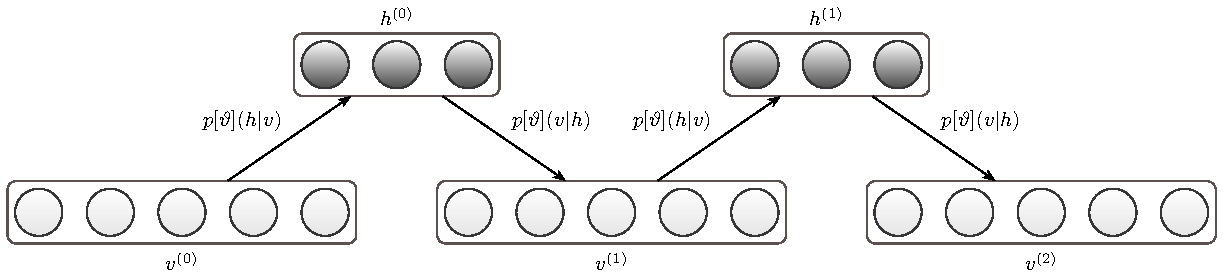
\includegraphics[width=\textwidth]{figures/gibbs-sampling-scheme.pdf}
      \end{center}
      \vfill
      \begin{itemize}
        \item to estimate $\expect_ϑ\boxBrackets{\mathscr{V}\transpose{\mathscr{H}}}$ perform Gibbs sampling
        \pause
        \item slow because it has to reach equilibrium
      \end{itemize}
    \end{frame}

    \begin{frame}{Learning: Contrastive Divergence}
      \begin{itemize}
        \item abort Gibbs Sampling after $v^{(k)}$ and $h^{(k)}$ are computed
        \pause
        \item approximate the expectation value
      \end{itemize}
      \pause
      \vfill
      \begin{mybox}
        \[
          \expect_ϑ\boxBrackets{\mathscr{V}\transpose{\mathscr{H}}} \approx v^{(k)}\transpose{h^{(k)}}
        \]
      \end{mybox}
    \end{frame}

    \begin{frame}{Learning: Example}
      \begin{center}
        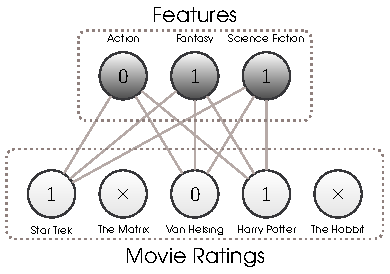
\includegraphics[scale=1.0]{figures/rbm-learning-example.pdf}
      \end{center}
      \vfill
      \begin{itemize}
        \pause
        \item one RBM for every user with connections for rated movies
        \pause
        \item weights and biases off all RBM are tied together
      \end{itemize}
    \end{frame}
  % section Learning (end)

  \section{Inference} % (fold)
  \label{sec:inference}
    \begin{frame}{Inference: Example}
      \begin{center}
        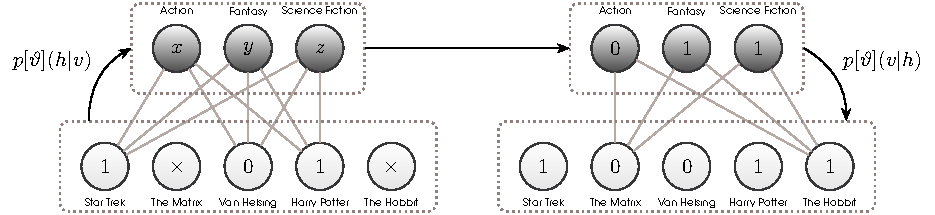
\includegraphics[width=\textwidth]{figures/rbm-inference-example.pdf}
      \end{center}
      \vfill
      \begin{itemize}
        \pause
        \item compute hidden values only for rated movies
        \pause
        \item compute visible values of unrated movies based on hidden values
      \end{itemize}
    \end{frame}
  % section inference (end)

  % \section{Implementation} % (fold)
  % \label{sec:implementation}
  %   \begin{frame}{Implementation}

  %   \end{frame}
  % % section implementation (end)

  \section{Results} % (fold)
  \label{sec:results}
    \begin{frame}{Results: MovieLens Dataset by GroupLens}
      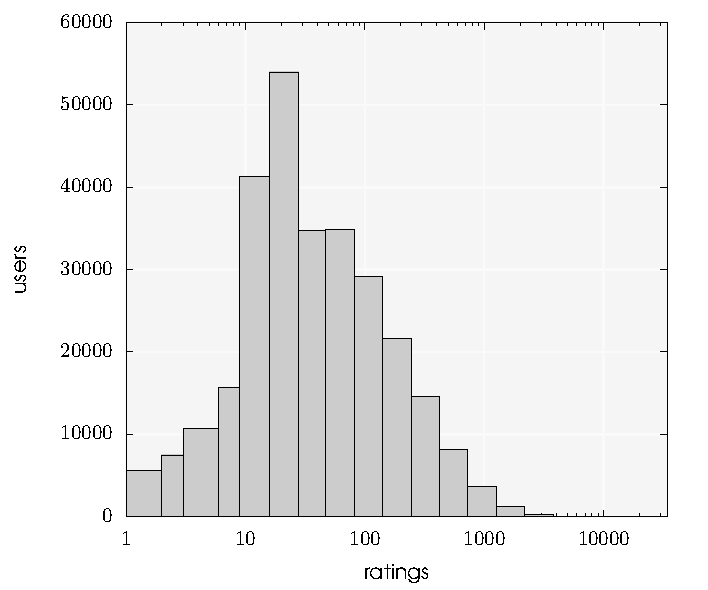
\includegraphics[width=0.45\textwidth]{figures/movielens-user-histogram.pdf}
      \hfill
      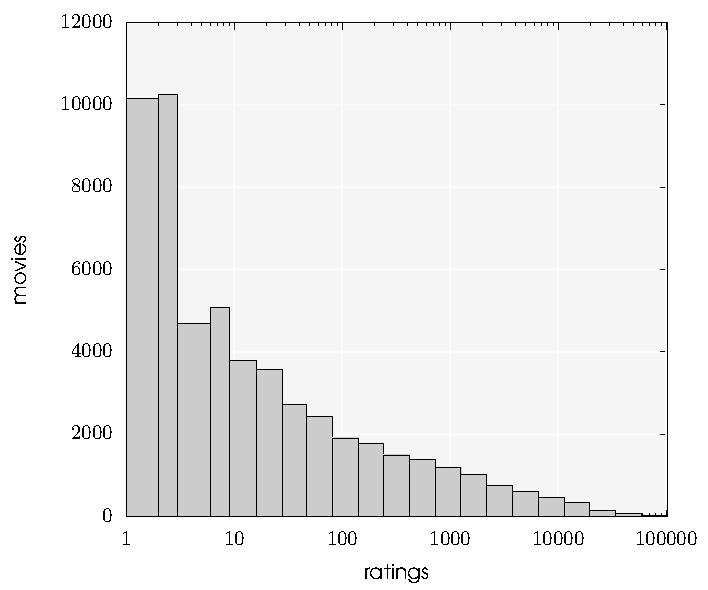
\includegraphics[width=0.45\textwidth]{figures/movielens-movie-histogram.pdf}
      \vfill
      \begin{itemize}
        \item $\sim$ 27,000,000 ratings, $\sim$ 58,000 movies, $\sim$ 280,000 users
        \item current implementation not completely tested \\ ($\sim 80\%$ correct predictions)
      \end{itemize}
    \end{frame}
  % section results (end)

  \section{Going Further} % (fold)
  \label{sec:Going Further}
    \begin{frame}{Going Further: Tweak the Learning}
      \begin{itemize}
        \item Contrastive Divergence Variants
        \item Momentum
        \item Weight Decay
        \item Different types of units
      \end{itemize}
    \end{frame}

    \begin{frame}{Going Further: Applications}
      \begin{itemize}
        \item language modeling and document retrieval
        \item classification
        \item reducing dimensionality of data
      \end{itemize}
    \end{frame}
  % section Going Further (end)

  \begin{frame}
    \frametitle{References}
    \tiny
    \begin{multicols}{2}
      \nocite{*}
      \bibliography{references}
    \end{multicols}
  \end{frame}
\end{document}